\documentclass{beamer}

\usepackage{ucs}
\usepackage[utf8x]{inputenc}
\usepackage[T1]{fontenc}
\usepackage[english]{babel}
\usepackage{epstopdf}

%\usepackage{multirow}%	multirow
%\usepackage[retainorgcmds]{IEEEtrantools}%	IEEEeqnarray
%\usepackage{mathabx}%	convolution symbol
\usepackage{relsize}%	relative font sizes
%\usepackage{listings}
%\usepackage{graphicx}
\usepackage{multicol}
\usepackage{todonotes}
\usepackage{tangocolors}
\usepackage{tikz}
%\usepackage{enumitem}
%\usepackage{pgflibrarytikzbackgrounds}


%	presentation info
\title{A finite volume case study}

\subtitle{MPI: Implementation and Analysis}

\author{M. Palhas \and P. Costa}

\institute[19808 \and 19830]{
	University of Minho\\
	Department of Informatics
}

\date{Braga, April 2012}


%	beamer options
\usetheme{CambridgeUS}


\begin{document}%	begin presentation

\begin{frame}[plain]
	\titlepage
\end{frame}

\begin{frame}
	\frametitle{Index}
	\tableofcontents
\end{frame}



%
%
% MESH PARTITIONING: THE PROBLEM
%
%

\section{Mesh Partitioning}

\subsection{The Problem}

\begin{frame}
	\frametitle{Mesh Partitioning: The Problem}

	\begin{block}{Objective}
		\begin{enumerate}\itemsep=10pt
			\item Divide the mesh into $P$ partitions
			\pause
			\item Achieve good balance between partition sizes
			\pause
			\item Keep information about how they connect
			\pause
			\item Minimize border between them, without compromising (2)
		\end{enumerate}
	\end{block}


\end{frame}




%
%
% RESULTS
%
%

\subsection{Implementation}

\begin{frame}
	\frametitle{Mesh Partitioning: Implementation}

	Division of the mesh based only on $x$ coordinate of cells:
	\begin{enumerate}
		\item Create ordered set of cells (key is $x$ coord)
		\item Sequentially assing $N/P$ cells to each process
	\end{enumerate}

	\begin{figure}
		\begin{center}
			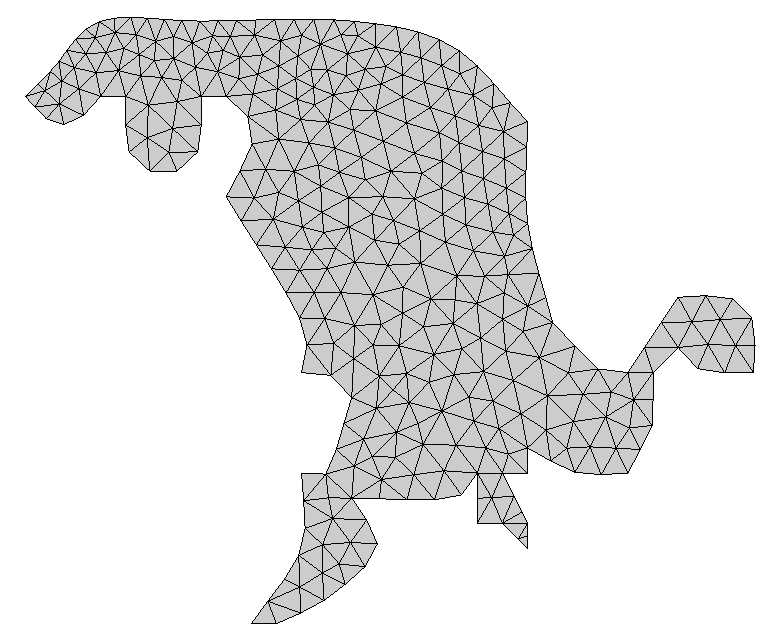
\includegraphics[width=0.45\columnwidth]{report.may/images/foz_msh}
		\end{center}
	\end{figure}
\end{frame}

\begin{frame}
	\frametitle{Mesh Partitioning: Implementation}

	Division of the mesh based only on $x$ coordinate of cells:
	\begin{enumerate}
		\item Create ordered set of cells (key is $x$ coord)
		\item Sequentially assing $N/P$ cells to each process.
	\end{enumerate}

	\begin{multicols}{2}
		\begin{figure}
			\begin{center}
				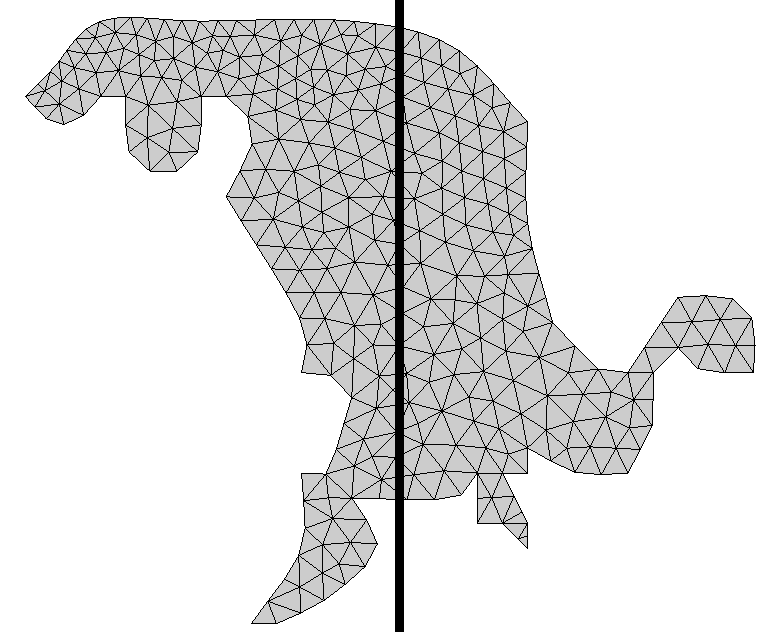
\includegraphics[width=0.955\columnwidth]{report.may/images/foz_p2_msh}
			\end{center}
		\end{figure}
		\begin{figure}
			\begin{center}
				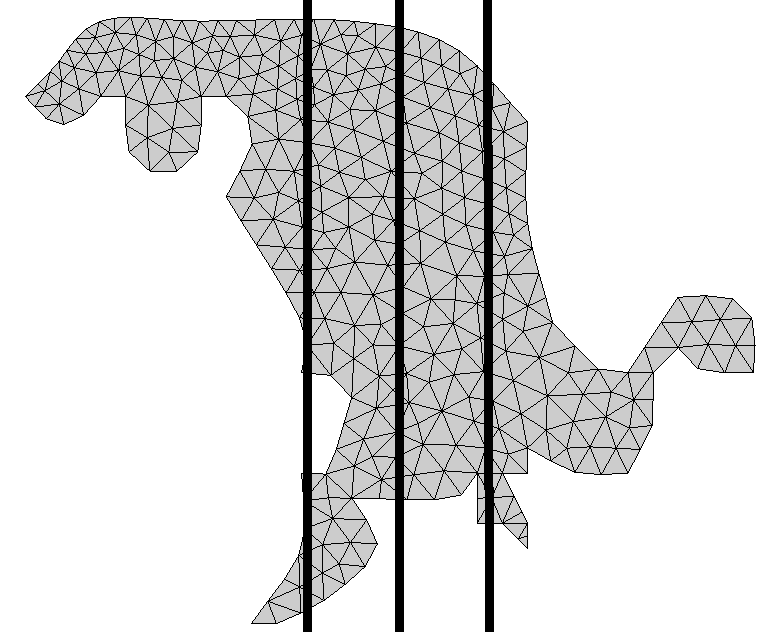
\includegraphics[width=0.955\columnwidth]{report.may/images/foz_p4_msh}
			\end{center}
		\end{figure}
	\end{multicols}
\end{frame}

\begin{frame}
\frametitle{Mesh Partitioning: Implementation}

	\begin{block}{Advantages}
		\begin{enumerate}\itemsep=10pt
			\item Simple concept and implementation
			\pause
			\item Each partition has at most a left and a right neighbour
			\begin{itemize}
				\item[-] Easy communication
			\end{itemize}
		\end{enumerate}
	\end{block}

	\pause
	\begin{block}{Disadvantages}
		\begin{enumerate}\itemsep=10pt
			\item Sequential sort and distribution are slow
			\pause
			\item No control over size of border between partitions (communication)
		\end{enumerate}
	\end{block}

\end{frame}



%
%
% TESTING METHODOLOGY
%
%

\section{Profiling}

\begin{frame}
	\frametitle{Index}
	\tableofcontents[currentsection]
\end{frame}

\subsection{Methodology}
\begin{frame}
%	\frametitle{Methodology}
	\begin{block}{Environmental Setup}
		\begin{itemize}
			\item{SeARCH Group 101
			\begin{description}
				\item{64-bit Intel\textregistered Xeon\texttrademark @ 3.2 GHz;}
				\item{4 threads per node;}
				\item{16 KB L1 data cache, 2 MB L2 cache, 2 GB RAM;}
			\end{description}
			}
			\item{6 nodes (21 to 26);}
		\end{itemize}
	\end{block}
	\pause
	\begin{block}{Methodology}
		\begin{itemize}
			\item{Three timers per version:
			\begin{enumerate}
				\setcounter{enumi}{-1}
				\item{Full program;}
				\item{Main loop;}
				\item{Functions;}
			\end{enumerate}
			}
			\item{2000 iterations;}
			\item{10 executions per timer.}
		\end{itemize}
	\end{block}
\end{frame}



%
%
% RESULTS
%
%

\section{Results}

\begin{frame}
	\frametitle{Index}
	\tableofcontents[currentsection]
\end{frame}



\subsection{Speedups}
\begin{frame}
	\todo[inline]{Add speedup graph}
\end{frame}



\subsection{Execution times}
\begin{frame}
	\todo[inline]{Add bathtub graph}
\end{frame}



\subsection{Bottlenecks}
\begin{frame}
	\todo[inline]{Add bathtub graph}
\end{frame}



%
%
% CONCLUSIONS
%
%

\section{Conclusions}

\begin{frame}
	\frametitle{Index}
	\tableofcontents[currentsection]
\end{frame}

\begin{frame}
	\todo[inline]{Add Stuff}

\end{frame}

\section{} % To hide "Conclusions" from the header of the last slide

\begin{frame}[plain]
	\titlepage
	\begin{center}
		\Huge\bfseries - ? -
	\end{center}
\end{frame}

\end{document}%	end presentation
